\section{Development process}


The development process has been agile in nature, with a weekly status meeting every Monday, where our progress was examined, and the next week planed. The meeting took the shape of a retrospective combined with planing, regularly taking 2-3 hours, as the previous weeks work and the challenges we had met was discussed and our requirements were reviewed in the light of the knowledge gained during the preceding week.

\begin{figure}[h]
\centering
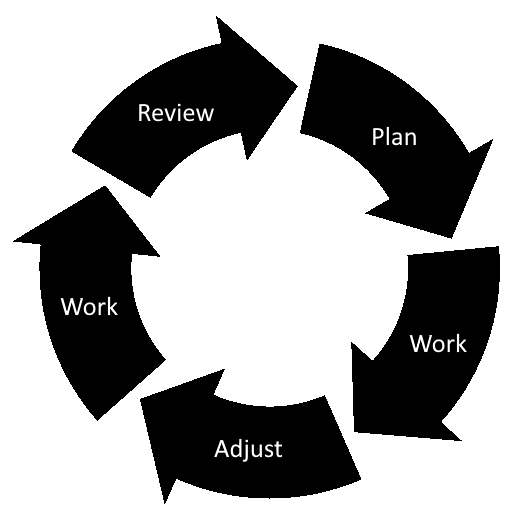
\includegraphics[scale=0.5]{02-Body/Images/WorkIterations.png}
\label{fig:iterate}
\caption{Illustration of work iteration}
\end{figure}

Once the tasks of the coming week had been decided and assigned, we worked individually, meeting again Wednesday morning for a supervisor meeting, which often took the shape of a short recap of our progress and a discussion with our supervisor, getting a fresh perspective on our solutions and challenges. Following the supervisor meeting we adjusted the planed tasks, taking the new perspective into consideration.

The adjusted tasks were then worked on until the next Monday meeting, resulting in an iterative process as illustrated in figure \ref{fig:iterate}.

